\documentclass{standalone}
\usepackage{tikz}
\usetikzlibrary{patterns, positioning}

\begin{document}
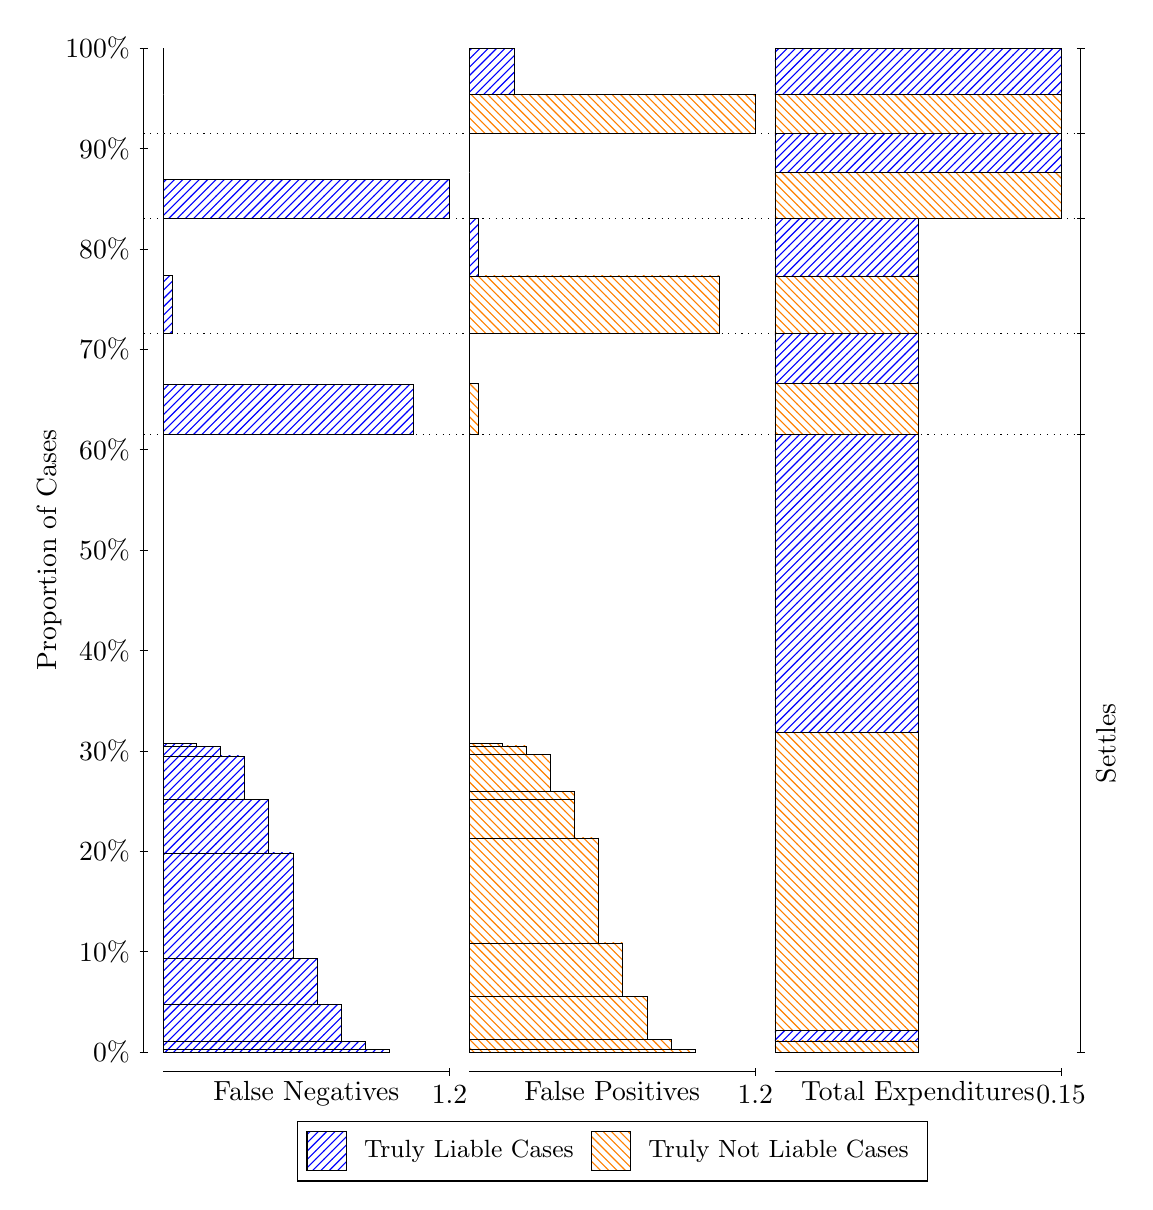
\begin{tikzpicture}
\draw[black, very thin] (1.5,1.75) -- (1.5,14.5);
\node[rotate=90, anchor=center] at (0.3, 8.125) {Proportion of Cases};
\draw[black, very thin] (1.45,1.75) -- (1.55,1.75);
\node[anchor=east] at (1.45, 1.75) {0\%};
\draw[black, very thin] (1.45,3.025) -- (1.55,3.025);
\node[anchor=east] at (1.45, 3.025) {10\%};
\draw[black, very thin] (1.45,4.3) -- (1.55,4.3);
\node[anchor=east] at (1.45, 4.3) {20\%};
\draw[black, very thin] (1.45,5.575) -- (1.55,5.575);
\node[anchor=east] at (1.45, 5.575) {30\%};
\draw[black, very thin] (1.45,6.85) -- (1.55,6.85);
\node[anchor=east] at (1.45, 6.85) {40\%};
\draw[black, very thin] (1.45,8.125) -- (1.55,8.125);
\node[anchor=east] at (1.45, 8.125) {50\%};
\draw[black, very thin] (1.45,9.4) -- (1.55,9.4);
\node[anchor=east] at (1.45, 9.4) {60\%};
\draw[black, very thin] (1.45,10.675) -- (1.55,10.675);
\node[anchor=east] at (1.45, 10.675) {70\%};
\draw[black, very thin] (1.45,11.95) -- (1.55,11.95);
\node[anchor=east] at (1.45, 11.95) {80\%};
\draw[black, very thin] (1.45,13.225) -- (1.55,13.225);
\node[anchor=east] at (1.45, 13.225) {90\%};
\draw[black, very thin] (1.45,14.5) -- (1.55,14.5);
\node[anchor=east] at (1.45, 14.5) {100\%};

\draw[black, very thin] (13.4,1.75) -- (13.4,14.5);
\draw[black, very thin] (13.35,1.75) -- (13.45,1.75);
\node[anchor=west] at (13.35, 1.75) {};
\draw[black, very thin] (13.35,9.5903) -- (13.45,9.5903);
\node[anchor=west] at (13.35, 9.5903) {};
\draw[black, very thin] (13.35,10.878) -- (13.45,10.878);
\node[anchor=west] at (13.35, 10.878) {};
\draw[black, very thin] (13.35,12.336) -- (13.45,12.336);
\node[anchor=west] at (13.35, 12.336) {};
\draw[black, very thin] (13.35,13.417) -- (13.45,13.417);
\node[anchor=west] at (13.35, 13.417) {};
\draw[black, very thin] (13.35,14.5) -- (13.45,14.5);
\node[anchor=west] at (13.35, 14.5) {};

\draw[black, very thin, pattern color=blue, pattern=north east lines] (1.75,1.75) rectangle (4.6184,1.7842);
\draw[black, very thin, pattern color=blue, pattern=north east lines] (1.75,1.7842) rectangle (4.3125,1.886);
\draw[black, very thin, pattern color=blue, pattern=north east lines] (1.75,1.886) rectangle (4.0065,2.3551);
\draw[black, very thin, pattern color=blue, pattern=north east lines] (1.75,2.3551) rectangle (3.7005,2.9413);
\draw[black, very thin, pattern color=blue, pattern=north east lines] (1.75,2.9413) rectangle (3.3946,4.2771);
\draw[black, very thin, pattern color=blue, pattern=north east lines] (1.75,4.2771) rectangle (3.0886,4.9605);
\draw[black, very thin, pattern color=blue, pattern=north east lines] (1.75,4.9605) rectangle (2.7826,5.5098);
\draw[black, very thin, pattern color=blue, pattern=north east lines] (1.75,5.5098) rectangle (2.4767,5.6323);
\draw[black, very thin, pattern color=blue, pattern=north east lines] (1.75,5.6323) rectangle (2.1707,5.6689);
\draw[black, very thin, pattern color=orange, pattern=north west lines] (1.75,5.6689) rectangle (1.75,9.5903);
\draw[black, very thin, pattern color=blue, pattern=north east lines] (1.75,9.5903) rectangle (4.9244,10.229);
\draw[black, very thin, pattern color=orange, pattern=north west lines] (1.75,10.229) rectangle (1.75,10.878);
\draw[black, very thin, pattern color=blue, pattern=north east lines] (1.75,10.878) rectangle (1.8647,11.608);
\draw[black, very thin, pattern color=orange, pattern=north west lines] (1.75,11.608) rectangle (1.75,12.336);
\draw[black, very thin, pattern color=blue, pattern=north east lines] (1.75,12.336) rectangle (5.3833,12.836);
\draw[black, very thin, pattern color=orange, pattern=north west lines] (1.75,12.836) rectangle (1.75,13.417);
\draw[black, very thin, pattern color=orange, pattern=north west lines] (1.75,13.417) rectangle (1.75,13.911);
\draw[black, very thin, pattern color=blue, pattern=north east lines] (1.75,13.911) rectangle (1.75,14.5);
\draw[black, very thin, pattern color=orange, pattern=north west lines] (5.6333,1.75) rectangle (8.5018,1.7869);
\draw[black, very thin, pattern color=orange, pattern=north west lines] (5.6333,1.7869) rectangle (8.1958,1.909);
\draw[black, very thin, pattern color=orange, pattern=north west lines] (5.6333,1.909) rectangle (7.8898,2.4552);
\draw[black, very thin, pattern color=orange, pattern=north west lines] (5.6333,2.4552) rectangle (7.5839,3.1352);
\draw[black, very thin, pattern color=orange, pattern=north west lines] (5.6333,3.1352) rectangle (7.2779,4.4678);
\draw[black, very thin, pattern color=orange, pattern=north west lines] (5.6333,4.4678) rectangle (6.9719,4.9603);
\draw[black, very thin, pattern color=orange, pattern=north west lines] (5.6333,4.9603) rectangle (6.9719,5.0567);
\draw[black, very thin, pattern color=orange, pattern=north west lines] (5.6333,5.0567) rectangle (6.666,5.5312);
\draw[black, very thin, pattern color=orange, pattern=north west lines] (5.6333,5.5312) rectangle (6.36,5.6362);
\draw[black, very thin, pattern color=orange, pattern=north west lines] (5.6333,5.6362) rectangle (6.054,5.6715);
\draw[black, very thin, pattern color=blue, pattern=north east lines] (5.6333,5.6715) rectangle (5.6333,9.5903);
\draw[black, very thin, pattern color=orange, pattern=north west lines] (5.6333,9.5903) rectangle (5.7481,10.24);
\draw[black, very thin, pattern color=blue, pattern=north east lines] (5.6333,10.24) rectangle (5.6333,10.878);
\draw[black, very thin, pattern color=orange, pattern=north west lines] (5.6333,10.878) rectangle (8.8077,11.607);
\draw[black, very thin, pattern color=blue, pattern=north east lines] (5.6333,11.607) rectangle (5.7481,12.336);
\draw[black, very thin, pattern color=orange, pattern=north west lines] (5.6333,12.336) rectangle (5.6333,12.918);
\draw[black, very thin, pattern color=blue, pattern=north east lines] (5.6333,12.918) rectangle (5.6333,13.417);
\draw[black, very thin, pattern color=orange, pattern=north west lines] (5.6333,13.417) rectangle (9.2667,13.911);
\draw[black, very thin, pattern color=blue, pattern=north east lines] (5.6333,13.911) rectangle (6.207,14.5);
\draw[black, very thin, pattern color=orange, pattern=north west lines] (9.5167,1.75) rectangle (11.333,1.8902);
\draw[black, very thin, pattern color=blue, pattern=north east lines] (9.5167,1.8902) rectangle (11.333,2.0263);
\draw[black, very thin, pattern color=orange, pattern=north west lines] (9.5167,2.0263) rectangle (11.333,5.8075);
\draw[black, very thin, pattern color=blue, pattern=north east lines] (9.5167,5.8075) rectangle (11.333,9.5903);
\draw[black, very thin, pattern color=orange, pattern=north west lines] (9.5167,9.5903) rectangle (11.333,10.24);
\draw[black, very thin, pattern color=blue, pattern=north east lines] (9.5167,10.24) rectangle (11.333,10.878);
\draw[black, very thin, pattern color=orange, pattern=north west lines] (9.5167,10.878) rectangle (11.333,11.607);
\draw[black, very thin, pattern color=blue, pattern=north east lines] (9.5167,11.607) rectangle (11.333,12.336);
\draw[black, very thin, pattern color=orange, pattern=north west lines] (9.5167,12.336) rectangle (13.15,12.918);
\draw[black, very thin, pattern color=blue, pattern=north east lines] (9.5167,12.918) rectangle (13.15,13.417);
\draw[black, very thin, pattern color=orange, pattern=north west lines] (9.5167,13.417) rectangle (13.15,13.911);
\draw[black, very thin, pattern color=blue, pattern=north east lines] (9.5167,13.911) rectangle (13.15,14.5);
\draw[black, dotted] (1.5,9.5903) -- (13.4,9.5903);
\draw[black, dotted] (1.5,10.878) -- (13.4,10.878);
\draw[black, dotted] (1.5,12.336) -- (13.4,12.336);
\draw[black, dotted] (1.5,13.417) -- (13.4,13.417);
\draw[black, very thin] (1.75,1.5) -- (5.3833,1.5);
\node[anchor=north] at (3.5667, 1.5) {False Negatives};
\draw[black, very thin] (5.3833,1.45) -- (5.3833,1.55);
\node[anchor=north] at (5.3833, 1.45) {1.2};

\draw[black, very thin] (5.6333,1.5) -- (9.2667,1.5);
\node[anchor=north] at (7.45, 1.5) {False Positives};
\draw[black, very thin] (9.2667,1.45) -- (9.2667,1.55);
\node[anchor=north] at (9.2667, 1.45) {1.2};

\draw[black, very thin] (9.5167,1.5) -- (13.15,1.5);
\node[anchor=north] at (11.333, 1.5) {Total Expenditures};
\draw[black, very thin] (13.15,1.45) -- (13.15,1.55);
\node[anchor=north] at (13.15, 1.45) {0.15};

\node[black, centered, rotate=90] at (13.72, 5.6702) {Settles};





\draw (7.449999999999999,1.5) node[draw=none] (baseCoordinate) {};
\begin{scope}[align=center]
        \matrix[scale=0.5, draw=black, below=0.5cm of baseCoordinate, nodes={draw}, column sep=0.1cm]{
            \node[rectangle, draw, minimum width=0.5cm, minimum height=0.5cm, pattern=north east lines, pattern color=blue] {}; &
            \node[draw=none, font=\small] (B) {Truly Liable Cases}; &
            \node[rectangle, draw, minimum width=0.5cm, minimum height=0.5cm, pattern=north west lines, pattern color=orange] {}; &
            \node[draw=none, font=\small] (B) {Truly Not Liable Cases}; \\
            };
\end{scope}

\end{tikzpicture}
\end{document}